

\subsection{Efecto Ramsauer--Townsend}

Las Figuras~\ref{auto} y
\ref{manual} muestran los voltajes de ánodo \(V_a\) y de
rejilla-blindaje \(V_{rb}\) en función del voltaje de cátodo \(V_c\), para
voltajes de filamento de \(V_f=2\), \(3\) y \(4~\mathrm{V}\). La primera
corresponde a la adquisición realizada mediante el software del laboratorio,
mientras que la segunda contiene las mediciones efectuadas manualmente.

\begin{figure*}
    \centering
    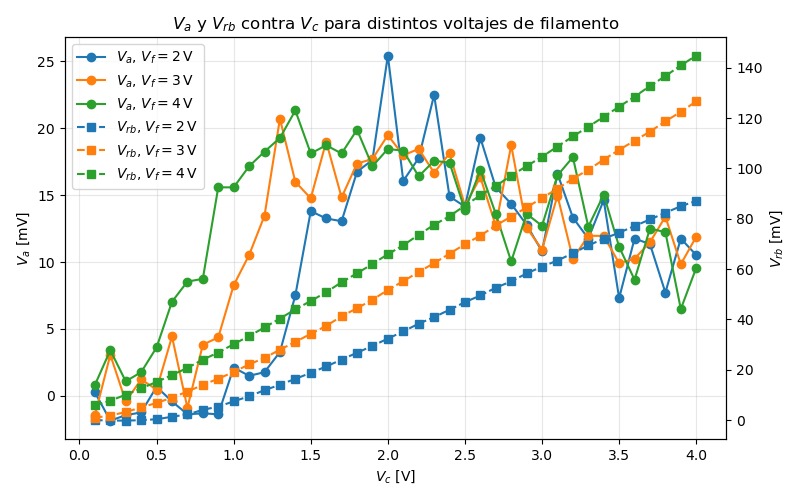
\includegraphics[width=\linewidth]{figuras/va_vrb_vs_vc_utomatico.png}
    \captionof{figure}{Resultados de las mediciones usando el software del laboratorio.}
    \label{auto}
\end{figure*}

\begin{figure*}
    \centering
    
\includegraphics[width=\linewidth]{figuras/va_vrb_vs_vc_una_grafica.png}
    \captionof{figure}{Resultados de las mediciones en modalidad manual.}
    \label{manual}
\end{figure*}

\subsection{Técnica de Townsend pulsada}

La velocidad de deriva electrónica \(v_{\mathrm d}\), calculada a partir
del tiempo de tránsito medido en el osciloscopio, se presenta en la
Figura~\ref{v_contra_Tausen} como función del campo eléctrico reducido
\(E/N\). Los datos corresponden a presiones comprendidas entre
aproximadamente \(10.1\) y \(200~\mathrm{Torr}\).

\begin{figure*}
    \centering
    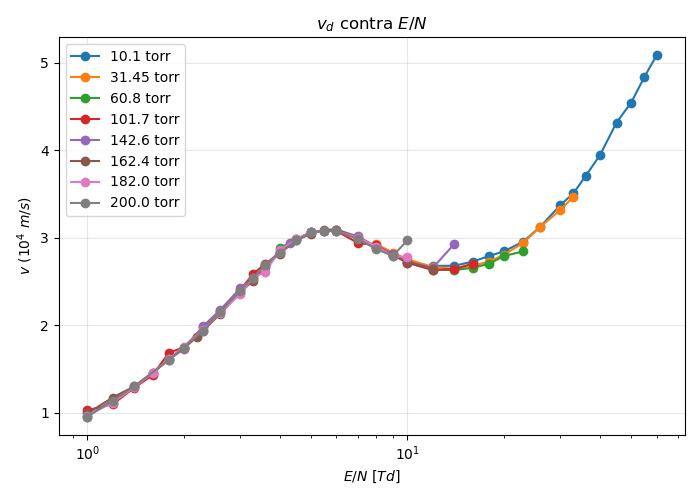
\includegraphics[width=\linewidth]{figuras/v_contraEN.png}
    \captionof{figure}{Velocidad de deriva en función del campo eléctrico reducido \(E/N\) para cada presión estudiada.}
    \label{v_contra_Tausen}
\end{figure*}